\section{Conexión por arcos}

\begin{ejercicio}
    Muestra que cualquier esfera de $\mathbb{R}^n$, $n\geq 2$ es arcoconexa con la topología usual.\\

    \noindent
    Es decir, queremos ver que $\bb{S}^n$ es arcoconexa para $n\geq 1$. \newline (notemos que $\bb{S}^0 = \{x\in \mathbb{R} : \|x\| = 1\} = \{-1,1\}$ no es un conjunto arcoconexo).\\

    \noindent
    Para ello, sea $n\geq 2$, sabemos que $\bb{S}^n\setminus\{p\}$ (con $p\in \bb{S}^n$) es homeomorfa a $\mathbb{R}^{n-1}$, que es un conjunto arcoconexo por ser convexo (es una espacio vectorial). Como la arcoconexión es una propiedad topológica, esta se conserva por homeomorfismo, luego $\bb{S}^n\setminus \{p\}$ es un conjunto arcoconexo, $\forall p\in \bb{S}^n$.

    Tomando $N = (0,\ldots,0,1), S =(0,\ldots,0,-1) \in \bb{S}^n$, podemos ver $\bb{S}^n$ como unión de dos conjuntos arcoconexos:
    \begin{equation*}
        \bb{S}^n = (\bb{S}^n\setminus\{N\}) \cup (\bb{S}^n\setminus\{S\})
    \end{equation*}

    no disjuntos:
    \begin{equation*}
        (\bb{S}^n\setminus\{N\}) \cap (\bb{S}^n\setminus\{S\}) = \bb{S}^n\setminus\{N,S\}
    \end{equation*}
    Por lo que $\bb{S}^n$ es un conjunto arcoconexo, $\forall n\geq 2$.
\end{ejercicio}

\begin{ejercicio}
    Demuestra que si $\{A_i\}_{i \in I}$ es una familia de arcoconexos de $X$ tales que todos intersecan a uno de ellos, es decir,
    \begin{equation*}
        A_i\cap A_{i_0} \neq \emptyset, \qquad \forall i \in I,
    \end{equation*}
    entonces $\bigcup\limits_{i \in I}A_i$ es arcoconexo.\\

    \noindent
    Sean $x,y\in \bigcup\limits_{i \in I}A_i$, entonces existen $i,j\in I$ de forma que $x\in A_i$ y $y\in A_j$. Como $A_i \cap A_{i_0}, A_j\cap A_{i_0}\neq \emptyset $, podemos tomar $a\in A_i\cap A_{i_0}$ y $b\in A_j\cap A_{i_0}$.
    \begin{itemize}
        \item $A_i$ es un conjunto arcoconexo con $x,a\in A_i$, por lo que existe un camino, $\alpha$, que une $x$ con $a$.
        \item $A_j$ también es un conjunto arcoconexo con $y,b\in A_j$, por lo que existe un camino, $\beta$, que une $y$ con $b$.
        \item Además, $A_{i_0}$ es un conjunto arcoconexo con $a,b\in A_{i_0}$, por lo que existe un tercer camino, $\gamma$, que une $a$ con $b$.
    \end{itemize}
    De esta forma, podemos tomar:
    \begin{equation*}
        \sigma = \alpha \ast \left(\gamma \ast \tilde{\beta}\right)
    \end{equation*}
    Que es un camino que une $x$ con $y$. Como $x$ e $y$ eran arbitrarios, podemos unir cualesquiera dos puntos de $\bigcup\limits_{i \in I}A_i$, por lo que dicho conjunto es arcoconexo.

    \begin{figure}[H]
        \centering
        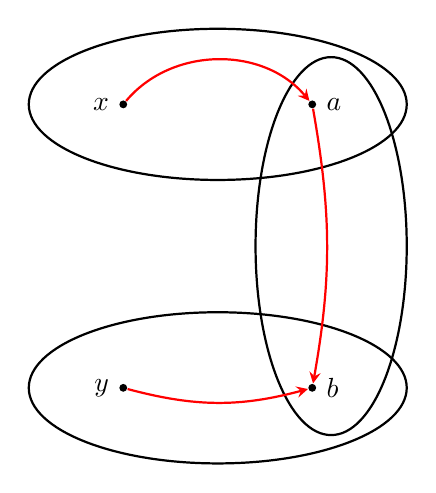
\begin{tikzpicture}[scale=1.2]
        % Dibujar elipses (conjuntos)
        \draw[thick] (0,1.5) ellipse (2 and 0.8); % elipse superior horizontal
        \draw[thick] (0,-1.5) ellipse (2 and 0.8); % elipse inferior horizontal
        \draw[thick] (1.2,0) ellipse (0.8 and 2);  % elipse vertical

        % Puntos
        \node[circle,fill=black,inner sep=1pt,label=left:$x$] (x) at (-1,1.5) {};
        \node[circle,fill=black,inner sep=1pt,label=right:$a$] (a) at (1,1.5) {};
        \node[circle,fill=black,inner sep=1pt,label=right:$b$] (b) at (1,-1.5) {};
        \node[circle,fill=black,inner sep=1pt,label=left:$y$] (y) at (-1,-1.5) {};

        % Arcos dirigidos
        \draw[-stealth,thick,red,bend left=50] (x) to (a);
        \draw[-stealth,thick,red,bend left=10] (a) to (b);
        \draw[-stealth,thick,red,bend right=15] (y) to (b);
        \end{tikzpicture}
        \caption{Forma de unir dos puntos cualesquiera.}
    \end{figure}
\end{ejercicio}

\begin{ejercicio}
    Sea $X$ un conjunto, $x_0\in X$, y consideramos la topología (del punto incluido) dada por
    \begin{equation*}
        T = \{U\subset X : x_0 \in U\} \cup \{\emptyset \}
    \end{equation*}
    ¿Es $(X,T)$ arcoconexo?\\

    \noindent
    Sí: sea $x\in X$, veamos que la aplicación $\alpha:[0,1]\to X$ dada por
    \begin{equation*}
        \alpha(t) = \left\{\begin{array}{ll}
                x & \text{si } t\in [0,\nicefrac{1}{2}] \\
                x_0 & \text{si } t\in \left]\nicefrac{1}{2},1\right]
        \end{array}\right. \qquad \forall t\in [0,1]
    \end{equation*}
    es continua. Sea $U\in T$:
    \begin{itemize}
        \item Si $U = \emptyset $, entonces $\alpha^{-1}(U) = \emptyset \in \cc{T}_u\big|_{[0,1]}$.
        \item Si $x_0\in U$ y $x\notin U$, entonces $\alpha^{-1}(U) = \left]\nicefrac{1}{2},1\right]\in \cc{T}_u\big|_{[0,1]}$.
        \item Si $x_0,x\in U$, entonces $\alpha^{-1}(U) = [0,1] \in \cc{T}_u\big|_{[0,1]}$.
    \end{itemize}
    Como la preimagen de cualquier conjunto abierto es abierta, tenemos que $\alpha$ es continua, luego es un arco que une $x$ con $x_0$.\\

    \noindent
    Ahora, si $x,y\in X$, tenemos que existen $\alpha,\beta:[0,1]\to X$ de forma que $\alpha$ une $x$ con $x_0$ y $\beta$ une $y$ con $x_0$; por lo que $\alpha\ast\tilde{\beta}$ es un arco que une $x$ con $y$. Como $x$ e $y$ eran arbitrarios, concluimos que $X$ es arcoconexo.
\end{ejercicio}

\begin{ejercicio}
   Demustra que en $\mathbb{R}^n$  con la topología usual, todo abierto conexo es arcoconexo. ¿Es cierto que todo cerrado conexo de $\mathbb{R}^n$ es arcoconexo?\\

   \noindent
   En teoría vimos que:
   \begin{equation*}
       \text{Un conjunto es arcoconexo} \Longleftrightarrow \left\{\begin{array}{l}
           \text{Es conexo} \\
           \text{Todo punto admite un entorno arcoconexo}
       \end{array}\right.
   \end{equation*}
   Sea $U$ un abierto conexo de $(\mathbb{R}^n, \cc{T}_u)$, falta ver que todo punto suyo admite un entorno arcoconexo en la topología inducida en $U$ para ver que $U$ es arcoconexo. Para ello, sea $x\in U$, como $U$ es abierto existe $r\in \mathbb{R}^+$ de forma que $B(x,r)\subset U$. $B(x,r)$ es un conjunto arcoconexo por ser convexo, luego es un entorno arcoconexo de $x$ en $U$. Como $x$ era un punto arbitrario de $U$, todo punto suyo admite un entorno arcoconexo, y como $U$ era conexo, tenemos que $U$ es arcoconexo.\\

   \noindent
   Ahora, no es cierto que todo cerrado conexo de $\mathbb{R}^n$ es arcoconexo, ya que si consideramos $f:\mathbb{R}^+\to \mathbb{R}$ dada por:
   \begin{equation*}
       f(x) = \sen\left(\dfrac{1}{x}\right) \qquad \forall x\in \mathbb{R}^+
   \end{equation*}
   Tenemos que
   \begin{equation*}
       C = \overline{Gr(f)} = \overline{\{(x,f(x)) : x\in \mathbb{R}^+\}} = Gr(f) \cup (\{0\}\times [-1,1])
   \end{equation*}
   es un conjunto cerrado y conexo (se vio en Topología I) pero que no es arcoconexo, puede probarse por un razonamiento similar a un ejemplo visto en teoría.

   \begin{figure}[H]
       \centering
        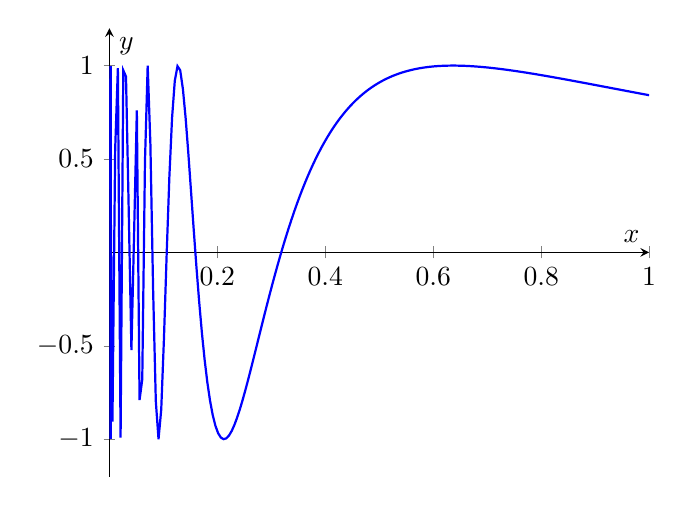
\begin{tikzpicture}
          \begin{axis}[
            axis lines=middle,
            xlabel={$x$}, ylabel={$y$},
            xmin=0, xmax=1,
            ymin=-1.2, ymax=1.2,
            samples=200 % menos puntos = compila más rápido
          ]
            \addplot[blue, thick, domain=0.0005:1] {sin(deg(1/x))};
            \addplot[blue, ultra thick] coordinates {(0,-1) (0,1)};
          \end{axis}
        \end{tikzpicture}
        \caption{Dibujo de la adherencia de la gráfica de $f(x)$.}
   \end{figure}
\end{ejercicio}

\begin{ejercicio}
    Prueba que la componente arcoconexa de un punto $x_0$ está contenida en la componente conexa de $x_0$.\\

    \noindent
    Sea $(X,T)$ un espacio topológico, $x_0\in X$ y $C$ la componente arcoconexa de $x_0$ en $X$, en particular tenemos que $C$ es un conjunto arcoconexo, luego es conexo, por lo que está contenida en la componente conexa de $x$, al ser esta el mayor conjunto conexo que contiene a $x$.
\end{ejercicio}

\begin{ejercicio}
    En $\mathbb{R}$ con la topología de Sorgenfrey, esto es, la topología que tiene como base
    \begin{equation*}
        \cc{B}_S = \{[a,b) \subset \mathbb{R} : a<b\},
    \end{equation*}
    determina sus componentes arcoconexas.\\

    \noindent
    En Topología I vimos que las componentes conexas de la topología de Sorgenfrey eran los conjuntos de puntos unitarios $\{x\}$, ya que si tenemos un conjunto $A\subset \mathbb{R}$ con al menos dos puntos distintos $x$ e $y$ (suponemos $x<y$), entonces en la topología inducida en $A$ podemos considerar los abiertos:
    \begin{equation*}
        U = [-\infty,y)\cap A, \qquad V = [y,+\infty)\cap A
    \end{equation*}
    de forma que $U,V\neq \emptyset $, $U\cup V = A$ y $U\cap V = \emptyset $, por lo que $A$ (cualquier conjunto con al menos dos puntos distintos) es disconexo, luego las componentes conexas han de ser los conjuntos unitarios, ya que los conjuntos unitarios son conexos en cualquier topología.

    Como las componentes arcoconexas se encuentran contenidas en las componentes conexas, no queda más salida que las componentes arcoconexas de la topología de Sorgenfrey sean los conjuntos unitarios.
\end{ejercicio}

\begin{ejercicio}
    Sea $f:X\to Y$ un homeomorfismo entre espacios topológicos. Demuestra que $A\subset X$ es una componente arcoconexa de $X$ si y solo si $f(X)$ es una componente arcoconexa de $Y$. Deduce que el número de componentes arcoconexas es invariante por homeomorfismos.\\

    \noindent
    Sea $A\subset X$ una componente arcoconexa de $X$, veamos que $f(A)$ es una componente arcoconexa de $Y$. Para ello, por reducción al absurdo, si $f(A)$ no fuera una componente arcoconexa de $Y$ podría ser por dos razones:
    \begin{itemize}
        \item $f(A)$ no es un conjunto arcoconexo, algo que llevaría a una contradicción, ya que se vio que la imagen por una función continua de un conjunto arcoconexo era arcoconexa.
        \item Porque existe $B\subset Y$ un conjunto arcoconexo distinto de $f(A)$ de forma que $f(A)\subset B\subset Y$. En dicho caso, si aplicamos $f^{-1}$ en la anterior inclusión tenemos que:
            \begin{equation*}
                f^{-1}(f(A)) = A \subset f^{-1}(B) \subset X
            \end{equation*}
            Por lo que tenemos $f^{-1}(B)$, un conjunto arcoconexo\footnote{por ser imagen por una función continua de un conjunto arcoconexo.} distinto de $A$ que contiene a $A$, luego $A$ no era una componentes arcoconexa de $X$, contradicción.
    \end{itemize}
    En definitiva, si $A\subset X$ es una componente arcoconexa entonces $f(A)$ también lo es de $Y$. Ahora, si $f(A)$ es una componente arcoconexa de $Y$, basta aplicar que $f^{-1}$ también es un homeomorfismo para concluir que $f^{-1}(f(A)) = A$ es una componente arcoconexa de $X$.\\

    \noindent
    Sea $Z$ un espacio topológico, notaremos en este ejercicio:
    \begin{equation*}
        \Gamma_Z = \{U\subset Z : U \text{\ es una componente arcoconexa de\ } Z\}
    \end{equation*}
    Recuperando el homeomorfismo $f:X\to Y$, definimos
    \Func{\Phi}{\Gamma_X}{\Gamma_Y}{U}{f(U)}
    \begin{itemize}
        \item $\Phi$ está bien definida (es decir, $f(U)\in \Gamma_Y$ para $U\in \Gamma_X$), ya que hemos visto que la imagen de una componente arcoconexa de $X$ es una componente arcoconexa de $Y$.
        \item $\Phi$ es inyectiva, ya que si $U,V\in \Gamma_X$ con $f(U)=f(V)$, entonces por ser $f$ inyectiva tenemos que $U=V$.
        \item $\Phi$ es sobreyectiva, ya que si $W\in \Gamma_Y$, entonces $f^{-1}(W)\in \Gamma_X$, con:
            \begin{equation*}
                \Phi(f^{-1}(W)) = f(f^{-1}(W)) = W
            \end{equation*}
    \end{itemize}
    Por ser $\Phi$ biyectiva concluimos que $|\Gamma_X| = |\Gamma_Y|$; es decir, el número de componentes arcoconexas es invariante por homeomorfismos.
\end{ejercicio}

\begin{ejercicio}
    En $X=\mathbb{R}\times \{0,1\}$ se considera la topología que tiene por base
    \begin{equation*}
        \cc{B} = \{\left]a,b\right[\times \{0,1\} : a<b\}.
    \end{equation*}
    Demuestra que $X$ es arcoconexo. ¿Es $X$ homeomorfo a $\mathbb{R}$ con la topología usual?\\

    \noindent
    Sean $\alpha=(x,a),\beta=(y,b)\in X$, vamos a tratar de crear un arco que una $\alpha$ con $\beta$:
    \begin{itemize}
        \item Si $a=b$, entonces $\gamma:[0,1]\to X$ dada por:
            \begin{equation*}
                \gamma(t) = ((1-t)x + ty, a) \qquad \forall t\in [0,1]
            \end{equation*}
            Es una aplicación continua, ya que si tomamos $B = \left]a,b\right[\times \{0,1\}\in \cc{B}$, tenemos:
            \begin{equation*}
                \gamma^{-1}(B) = \gamma^{-1}(\left]a,b\right[\times \{0\}) \text{\ abierto de\ } [0,1]
            \end{equation*}
            Ya que el conjunto $\left]a,b\right[\times \{0\}$ es un abierto para la topología usual y $\alpha$ es una aplicación continua para la topología usual.
        \item Si $\alpha = (0,0)$ y $\beta = (0,1)$, entonces si tomamos $\gamma:[0,1]\to X$ dada por:
            \begin{equation*}
                \gamma(t) = \left\{\begin{array}{ll}
                        \alpha & \text{si\ } 0 \leq t \leq \nicefrac{1}{2}\\
                        \beta & \text{si\ } \nicefrac{1}{2}<t \leq 1
                \end{array}\right.
            \end{equation*}
            tenemos que $\gamma$ es continua, ya que si $B = \left]a,b\right[\times \{0,1\}\in \cc{B}$, tenemos que:
            \begin{equation*}
                \gamma^{-1}(B) = \left\{\begin{array}{cl}
                        \emptyset & \text{si\ } 0 \notin \left]a,b\right[ \\
                        \left[0,1\right] & \text{si\ } 0 \in \left]a,b\right[
                \end{array}\right.
            \end{equation*}
        \item Una vez discutidos dichos casos, suponemos ahora que $\alpha=(x,0)$ y $\beta = (y,1)$ (en caso contrario, sustituimos los papeles de $\alpha$ y $\beta$), en cuyo caso:
            \begin{itemize}
                \item Sabemos de la existencia de un arco $\gamma$ que une $\alpha$ con $(0,0)$.
                \item Sabemos de la existencia de un arco $\tau$ que une $(0,0)$ con $(0,1)$.
                \item Sabemos de la existencia de un arco $\pi$ que une $\beta$ con $(0,1)$.
            \end{itemize}
            Si consideramos el arco $\gamma \ast (\tau \ast \tilde{\pi})$ obtenemos un arco que une $\alpha$ con $\beta$.
    \end{itemize} 
    Por tanto, $X$ es arcoconexo, ya que somos capaces de unir cualesquiera dos puntos distintos de $X$ por un arco.\\

    \noindent
    Ahora, para responder a la pregunta de si $(\mathbb{R},\cc{T}_u)$ es homeomorfo a $X$, la respuesta es que no, y tenemos dos formas de justificar la respuesta:
    \begin{description}
        \item [Opción 1.] Sabemos que $(\mathbb{R},\cc{T}_u)$ es $T2$ por ser un espacio topológico metrizable, mientras que podemos probar que $X$ no es $T2$, ya que no existen ningún par de abiertos disjuntos uno conteniendo a $(0,0)$ y otro conteniendo a $(0,1)$, puesto que si $U$ es un abierto de $X$ que contiene a $(0,0)$, entonces como $\cc{B}$ es una base, existen $a,b\in \mathbb{R}$ de forma que:
            \begin{equation*}
                (0,0) \in \left]a,b\right[\times \{0,1\} \subset U
            \end{equation*}
            Sin embargo, tendríamos entonces que $(0,1)\in \left]a,b\right[\times \{0,1\}$, de donde $(0,1)\in U$, por lo que $X$ no es T2 y como ser T2 es una propiedad topológica, dichos espacios no pueden ser homeomorfos.
        \item [Opción 2.] Otra forma sería suponer que son homeomorfos, con lo que existe un homeomorfismo $f:\mathbb{R}\to X$. Sea $p\in \mathbb{R}$, resulta entonces que $\mathbb{R}\setminus \{p\}$ es homeomorfo a $X\setminus \{(p,0)\}$, pero:
            \begin{itemize}
                \item $\mathbb{R}\setminus\{p\}$ no es arcoconexo.
                \item $X\setminus \{(p,0)\}$ sí es arcoconexo, ya que podemos hacer que cualquier curva ``salte'' a $(p,1)$ sin perder su continuidad, con lo que podemos seguir conectando dos puntos cualesquiera.
            \end{itemize}
    \end{description}
\end{ejercicio}

\begin{ejercicio}
    En $\mathbb{R}^3$ con la topología usual, calcula las componentes arcoconexas de
    \begin{equation*}
        X = \{x,y,z) \in \mathbb{R}^3 : xyz = 1\}
    \end{equation*}

    \noindent
    Notemos que como $xyz = 1$, ninguno de ellos puede ser igual a 0, por lo que:
    \begin{equation*}
        X = \left\{(x,y,z)\in \mathbb{R}^3 : z=\dfrac{1}{xy} ,\quad  xy\neq 0\right\}
    \end{equation*}
    Si tomamos:
    \begin{equation*}
        \Gamma = \left\{(x,y) \in \mathbb{R}^2 : xy \neq 0\right\} = \mathbb{R}^\ast \times \mathbb{R}^\ast
    \end{equation*}
    y definimos $f:\Gamma\to \mathbb{R}$ dada por:
    \begin{equation*}
        f(x,y) = \dfrac{1}{xy} \qquad \forall (x,y)\in \Gamma
    \end{equation*}
    Tenemos que $X = Gr(f)$. Por tanto, definiendo $h:\Gamma\to X$ por:
    \begin{equation*}
        h(x,y) = (x,y,f(x,y)) \qquad \forall (x,y)\in \Gamma
    \end{equation*}
    Obtenemos (como vimos en Topología I) un homeomorfismo entre $\Gamma$ y $X$. Como $\Gamma$ tiene 4 componentes arcoconexas:
    \begin{equation*}
        \mathbb{R}^+\times \mathbb{R}^+, \qquad \mathbb{R}^+\times \mathbb{R}^-, \qquad \mathbb{R}^-\times\mathbb{R}^-, \qquad \mathbb{R}^-\times\mathbb{R}^-
    \end{equation*}
    y las componentes arcoconexas se convervan por homeomorfismos tal y como acabamos de ver en el ejercicio 7, tenemos que:
    \begin{equation*}
        h(\mathbb{R}^+\times \mathbb{R}^+), \qquad h(\mathbb{R}^+\times \mathbb{R}^-), \qquad h(\mathbb{R}^-\times\mathbb{R}^-), \qquad h(\mathbb{R}^-\times\mathbb{R}^-)
    \end{equation*}
    son las componentes arcoconexas de $X$.
\end{ejercicio}

\begin{ejercicio} % // TODO: HACER
    En $\mathbb{R}^2$ con la topología usual consideremos las rectas horizontales $A_n = \mathbb{R}\times \{\nicefrac{1}{n}\}$, $B_n = \mathbb{R}\times \{\nicefrac{-1}{n}\}$ y el eje de ordenadas menos el origen, esto es, $C=\{0\}\times (\mathbb{R}\setminus \{0\})$. Calcula las componentes conexas y arcoconexas de
    \begin{equation*}
        X = \left(\bigcup_{n\in \mathbb{N}}A_n\right) \cup \left(\bigcup_{n\in \mathbb{N}}B_n\right) \cup C \cup \{(1,0)\}.
    \end{equation*}
\end{ejercicio}

